% GNUPLOT: LaTeX picture with Postscript
\begingroup
  \makeatletter
  \providecommand\color[2][]{%
    \GenericError{(gnuplot) \space\space\space\@spaces}{%
      Package color not loaded in conjunction with
      terminal option `colourtext'%
    }{See the gnuplot documentation for explanation.%
    }{Either use 'blacktext' in gnuplot or load the package
      color.sty in LaTeX.}%
    \renewcommand\color[2][]{}%
  }%
  \providecommand\includegraphics[2][]{%
    \GenericError{(gnuplot) \space\space\space\@spaces}{%
      Package graphicx or graphics not loaded%
    }{See the gnuplot documentation for explanation.%
    }{The gnuplot epslatex terminal needs graphicx.sty or graphics.sty.}%
    \renewcommand\includegraphics[2][]{}%
  }%
  \providecommand\rotatebox[2]{#2}%
  \@ifundefined{ifGPcolor}{%
    \newif\ifGPcolor
    \GPcolortrue
  }{}%
  \@ifundefined{ifGPblacktext}{%
    \newif\ifGPblacktext
    \GPblacktexttrue
  }{}%
  % define a \g@addto@macro without @ in the name:
  \let\gplgaddtomacro\g@addto@macro
  % define empty templates for all commands taking text:
  \gdef\gplbacktext{}%
  \gdef\gplfronttext{}%
  \makeatother
  \ifGPblacktext
    % no textcolor at all
    \def\colorrgb#1{}%
    \def\colorgray#1{}%
  \else
    % gray or color?
    \ifGPcolor
      \def\colorrgb#1{\color[rgb]{#1}}%
      \def\colorgray#1{\color[gray]{#1}}%
      \expandafter\def\csname LTw\endcsname{\color{white}}%
      \expandafter\def\csname LTb\endcsname{\color{black}}%
      \expandafter\def\csname LTa\endcsname{\color{black}}%
      \expandafter\def\csname LT0\endcsname{\color[rgb]{1,0,0}}%
      \expandafter\def\csname LT1\endcsname{\color[rgb]{0,1,0}}%
      \expandafter\def\csname LT2\endcsname{\color[rgb]{0,0,1}}%
      \expandafter\def\csname LT3\endcsname{\color[rgb]{1,0,1}}%
      \expandafter\def\csname LT4\endcsname{\color[rgb]{0,1,1}}%
      \expandafter\def\csname LT5\endcsname{\color[rgb]{1,1,0}}%
      \expandafter\def\csname LT6\endcsname{\color[rgb]{0,0,0}}%
      \expandafter\def\csname LT7\endcsname{\color[rgb]{1,0.3,0}}%
      \expandafter\def\csname LT8\endcsname{\color[rgb]{0.5,0.5,0.5}}%
    \else
      % gray
      \def\colorrgb#1{\color{black}}%
      \def\colorgray#1{\color[gray]{#1}}%
      \expandafter\def\csname LTw\endcsname{\color{white}}%
      \expandafter\def\csname LTb\endcsname{\color{black}}%
      \expandafter\def\csname LTa\endcsname{\color{black}}%
      \expandafter\def\csname LT0\endcsname{\color{black}}%
      \expandafter\def\csname LT1\endcsname{\color{black}}%
      \expandafter\def\csname LT2\endcsname{\color{black}}%
      \expandafter\def\csname LT3\endcsname{\color{black}}%
      \expandafter\def\csname LT4\endcsname{\color{black}}%
      \expandafter\def\csname LT5\endcsname{\color{black}}%
      \expandafter\def\csname LT6\endcsname{\color{black}}%
      \expandafter\def\csname LT7\endcsname{\color{black}}%
      \expandafter\def\csname LT8\endcsname{\color{black}}%
    \fi
  \fi
    \setlength{\unitlength}{0.0500bp}%
    \ifx\gptboxheight\undefined%
      \newlength{\gptboxheight}%
      \newlength{\gptboxwidth}%
      \newsavebox{\gptboxtext}%
    \fi%
    \setlength{\fboxrule}{0.5pt}%
    \setlength{\fboxsep}{1pt}%
    \definecolor{tbcol}{rgb}{1,1,1}%
\begin{picture}(7200.00,4320.00)%
    \gplgaddtomacro\gplbacktext{%
      \csname LTb\endcsname%%
      \put(1123,619){\makebox(0,0)[r]{\strut{}$635\cdot10^{-9}$}}%
      \csname LTb\endcsname%%
      \put(1123,963){\makebox(0,0)[r]{\strut{}$640\cdot10^{-9}$}}%
      \csname LTb\endcsname%%
      \put(1123,1308){\makebox(0,0)[r]{\strut{}$645\cdot10^{-9}$}}%
      \csname LTb\endcsname%%
      \put(1123,1652){\makebox(0,0)[r]{\strut{}$650\cdot10^{-9}$}}%
      \csname LTb\endcsname%%
      \put(1123,1997){\makebox(0,0)[r]{\strut{}$655\cdot10^{-9}$}}%
      \csname LTb\endcsname%%
      \put(1123,2341){\makebox(0,0)[r]{\strut{}$660\cdot10^{-9}$}}%
      \csname LTb\endcsname%%
      \put(1123,2686){\makebox(0,0)[r]{\strut{}$665\cdot10^{-9}$}}%
      \csname LTb\endcsname%%
      \put(1123,3030){\makebox(0,0)[r]{\strut{}$670\cdot10^{-9}$}}%
      \csname LTb\endcsname%%
      \put(1123,3374){\makebox(0,0)[r]{\strut{}$675\cdot10^{-9}$}}%
      \csname LTb\endcsname%%
      \put(1123,3719){\makebox(0,0)[r]{\strut{}$680\cdot10^{-9}$}}%
      \csname LTb\endcsname%%
      \put(1221,425){\makebox(0,0){\strut{}$50$}}%
      \csname LTb\endcsname%%
      \put(1736,425){\makebox(0,0){\strut{}$100$}}%
      \csname LTb\endcsname%%
      \put(2251,425){\makebox(0,0){\strut{}$150$}}%
      \csname LTb\endcsname%%
      \put(2766,425){\makebox(0,0){\strut{}$200$}}%
      \csname LTb\endcsname%%
      \put(3281,425){\makebox(0,0){\strut{}$250$}}%
      \csname LTb\endcsname%%
      \put(3796,425){\makebox(0,0){\strut{}$300$}}%
      \csname LTb\endcsname%%
      \put(4311,425){\makebox(0,0){\strut{}$350$}}%
      \csname LTb\endcsname%%
      \put(4826,425){\makebox(0,0){\strut{}$400$}}%
      \csname LTb\endcsname%%
      \put(5341,425){\makebox(0,0){\strut{}$450$}}%
      \csname LTb\endcsname%%
      \put(5856,425){\makebox(0,0){\strut{}$500$}}%
      \csname LTb\endcsname%%
      \put(6371,425){\makebox(0,0){\strut{}$550$}}%
      \csname LTb\endcsname%%
      \put(6886,425){\makebox(0,0){\strut{}$600$}}%
    }%
    \gplgaddtomacro\gplfronttext{%
      \csname LTb\endcsname%%
      \put(170,2169){\rotatebox{-270}{\makebox(0,0){\strut{}Wellenlänge $\lambda/\SI{}{m}$}}}%
      \csname LTb\endcsname%%
      \put(4053,135){\makebox(0,0){\strut{}Pixelkoordinate$/\textrm{Pixel}$}}%
      \csname LTb\endcsname%%
      \put(6123,3545){\makebox(0,0)[r]{\strut{}Datenpunkte}}%
      \csname LTb\endcsname%%
      \put(6123,3351){\makebox(0,0)[r]{\strut{}Anpassung $\lambda_\text{f}(x)$}}%
      \csname LTb\endcsname%%
      \put(4053,4009){\makebox(0,0){\strut{}Kalibraiton des 29488-A5 Spektrums mit $\chi^2/\textrm{ddof}=\SI{1.69E-02}{}$}}%
    }%
    \gplbacktext
    \put(0,0){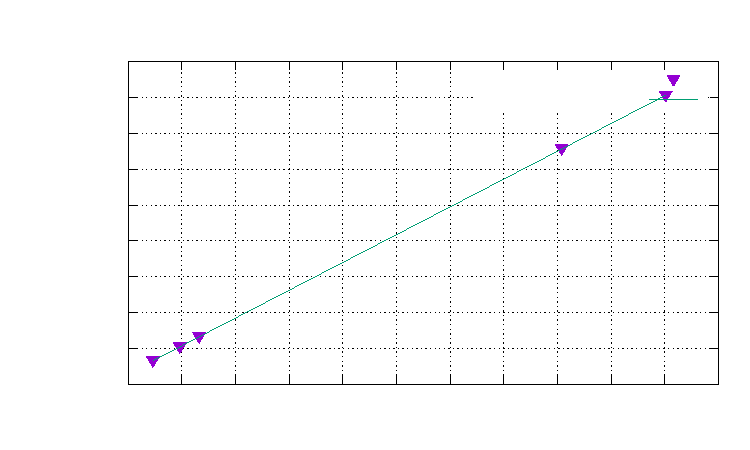
\includegraphics[width={360.00bp},height={216.00bp}]{29488-A5_kali}}%
    \gplfronttext
  \end{picture}%
\endgroup
